\chapter{TINJAUAN PUSTAKA}

\section{Koefisien Restitusi}

\subsection{Definisi dan Konsep Dasar}
Koefisien restitusi ($e$) merupakan parameter fundamental dalam mekanika yang mengukur tingkat elastisitas tumbukan antara dua benda. Parameter ini pertama kali diperkenalkan oleh Sir Isaac Newton melalui hukum restitusi Newton (\textit{Newton's law of restitution}) yang menyatakan bahwa rasio kecepatan pemisahan setelah tumbukan terhadap kecepatan pendekatan sebelum tumbukan adalah konstanta untuk material yang diberikan \citep{goldsmith1999theory}.

\subsection{Formulasi Matematis}
Secara matematis, koefisien restitusi didefinisikan sebagai persamaan yang menggambarkan hubungan antara kecepatan relatif sebelum dan setelah tumbukan. Diagram skematik pada Gambar \ref{fig:teori-figure-1} menunjukkan komponen kecepatan sebelum dan setelah tumbukan bola dengan permukaan datar.

\begin{figure}
    \centering
    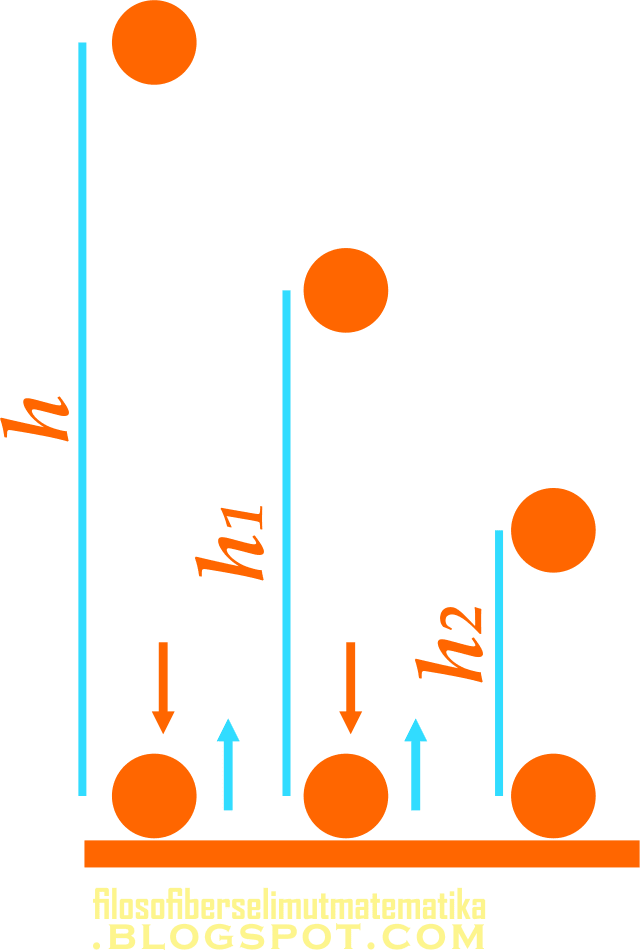
\includegraphics[width=0.3\linewidth]{images/gambar restitusi.png}
    \caption{Diagram skematik tumbukan bola dengan permukaan datar menunjukkan komponen kecepatan sebelum dan setelah tumbukan}
    \label{fig:teori-figure-1}
\end{figure}

\begin{equation}
    e = \frac{|v_{r}'|}{|v_{r}|} = \frac{|v_2' - v_1'|}{|v_1 - v_2|}
\end{equation}

dimana:
\begin{itemize}
    \item $e$ = koefisien restitusi (tanpa dimensi)
    \item $v_{r}'$ = kecepatan relatif setelah tumbukan (m/s)
    \item $v_{r}$ = kecepatan relatif sebelum tumbukan (m/s)
    \item $v_1', v_2'$ = kecepatan benda 1 dan 2 setelah tumbukan (m/s)
    \item $v_1, v_2$ = kecepatan benda 1 dan 2 sebelum tumbukan (m/s)
\end{itemize}

Untuk kasus khusus tumbukan vertikal dengan permukaan datar, koefisien restitusi dapat dihitung menggunakan persamaan yang menyederhanakan analisis menjadi hubungan antara ketinggian awal dan ketinggian pantulan:

\begin{equation}
    e = \sqrt{\frac{h_2}{h_1}}
\end{equation}

dimana:
\begin{itemize}
    \item $h_1$ = tinggi awal pelepasan benda (m)
    \item $h_2$ = tinggi pantulan maksimum setelah tumbukan (m)
\end{itemize}

\subsection{Klasifikasi Tumbukan Berdasarkan Nilai Koefisien Restitusi}
Berdasarkan nilai koefisien restitusi, tumbukan dapat diklasifikasikan menjadi tiga kategori utama yang mencerminkan karakteristik energi yang berbeda. Tumbukan elastis sempurna terjadi ketika nilai koefisien restitusi sama dengan satu ($e = 1$), di mana seluruh energi kinetik sistem terpelihara dan fenomena ini biasanya terjadi pada tumbukan antar partikel dalam kondisi ideal \citep{stronge2018impact}. Kondisi kedua adalah tumbukan tidak elastis sempurna dengan nilai koefisien restitusi nol ($e = 0$), di mana seluruh energi kinetik relatif dikonversi menjadi energi internal seperti panas dan deformasi permanen \citep{johnson1987contact}. Kategori ketiga merupakan tumbukan tidak elastis sebagian dengan rentang nilai antara nol dan satu ($0 < e < 1$), di mana sebagian energi kinetik hilang dalam proses tumbukan, dan kondisi ini merupakan fenomena umum dalam tumbukan nyata \citep{cross2002coefficient}.

\subsection{Hubungan koefisien restitusi dengan Sifat Material dan Deformasi}
Nilai koefisien restitusi bergantung pada karakteristik intrinsik material yang meliputi modulus elastisitas ($E$), batas luluh (\(\sigma_y\)), dan sifat viskoelastik material \citep{meyer2020coefficient}. Material dengan modulus elastisitas tinggi seperti baja atau keramik umumnya menunjukkan nilai $e$ yang lebih besar dibandingkan material dengan modulus rendah seperti polimer atau busa \citep{brancazio1981physics}. Proses deformasi selama tumbukan dapat dibagi menjadi dua fase yang saling berkaitan yaitu kompresi dan restorasi. Pada fase kompresi, energi kinetik dikonversi menjadi energi deformasi elastis dan plastis, sedangkan pada fase restorasi, energi deformasi elastis dikembalikan menjadi energi kinetik sementara energi deformasi plastis menjadi energi disipasi \citep{hartono2019analisis}.

\subsection{Faktor-Faktor yang Mempengaruhi Koefisien Restitusi}

Berbagai faktor mempengaruhi nilai koefisien restitusi dalam proses tumbukan nyata. Kecepatan tumbukan merupakan faktor pertama yang signifikan, di mana peningkatan kecepatan tumbukan menyebabkan deformasi plastis yang lebih besar sehingga menurunkan nilai $e$ \citep{smith2018experimental}. Karakteristik permukaan juga berperan penting, di mana kekasaran permukaan ($R_a$) dan kondisi pelumasan mempengaruhi energi disipasi melalui gesekan \citep{penner2002physics}. Temperatur lingkungan memberikan pengaruh terhadap sifat material, di mana peningkatan temperatur menurunkan modulus elastisitas material yang berdampak pada penurunan nilai $e$ \citep{lamb1945hydrodynamics}. Geometri benda turut mempengaruhi distribusi tegangan selama tumbukan, di mana bentuk dan ukuran relatif benda menentukan pola deformasi yang terjadi \citep{stronge2018impact}.

\section{Sensor Ultrasonik HC-SR04}

\subsection{Prinsip Kerja dan Teori Dasar}
Sensor ultrasonik HC-SR04 beroperasi berdasarkan prinsip \textit{time-of-flight} (TOF) menggunakan gelombang ultrasonik dengan frekuensi 40 kHz \citep{fauzi2020pengujian}. Prinsip kerja sensor ini mengikuti persamaan fundamental yang menghubungkan jarak dengan waktu tempuh gelombang:

\begin{equation}
    d = \frac{v \cdot t}{2}
\end{equation}

dimana:
\begin{itemize}
    \item $d$ = jarak objek dari sensor (m)
    \item $v$ = kecepatan suara dalam udara (m/s)
    \item $t$ = waktu tempuh gelombang ultrasonik (s)
    \item Faktor 2 dalam penyebut mengakibatkan perjalanan gelombang bolak-balik
\end{itemize}

Kecepatan suara dalam udara dapat dihitung menggunakan persamaan yang mempertimbangkan pengaruh temperatur lingkungan:

\begin{equation}
    v = 331.4 + 0.6 \cdot T
\end{equation}

dimana:
\begin{itemize}
    \item $T$ = temperatur udara dalam Celsius (°C)
    \item 331.4 = kecepatan suara pada 0°C (m/s)
    \item 0.6 = koefisien temperatur (m/s·°C)
\end{itemize}

\subsection{Spesifikasi Teknis}
Sensor HC-SR04 memiliki karakteristik teknis yang mendukung aplikasi pengukuran jarak dengan presisi tinggi \citep{siregar2021sensor}. Sensor ini beroperasi pada tegangan 5V DC dengan konsumsi arus sebesar 15 mA, memiliki rentang pengukuran dari 2 cm hingga 400 cm dengan akurasi ±3 mm. Sudut deteksi sensor mencapai 15° yang memungkinkan deteksi objek dalam area yang cukup luas, menggunakan frekuensi ultrasonik 40 kHz untuk transmisi gelombang, dan memerlukan durasi pulsa trigger minimum 10 $\mu$s untuk mengaktifkan proses pengukuran.

\subsection{Konfigurasi Pin dan Antarmuka}
Sensor HC-SR04 dirancang dengan empat pin utama yang masing-masing memiliki fungsi spesifik dalam sistem pengukuran. Pin VCC berfungsi sebagai input tegangan 5V DC untuk suplai daya sensor, pin GND merupakan ground atau referensi tegangan 0V, pin Trig adalah input untuk memicu pengiriman gelombang ultrasonik, dan pin Echo adalah output yang memberikan pulsa dengan lebar yang sebanding dengan jarak objek yang dideteksi. Konfigurasi pin ini ditunjukkan pada Gambar \ref{fig:teori-figure-2} yang menggambarkan diagram pin dan konfigurasi sensor ultrasonik HC-SR04.

\begin{figure}
    \centering
    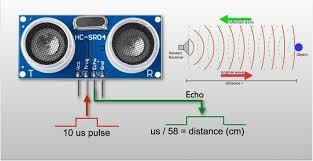
\includegraphics[width=0.5\linewidth]{images/hcsr.jpg}
    \caption{Diagram pin dan konfigurasi sensor ultrasonik HC-SR04}
    \label{fig:teori-figure-2}
\end{figure}

\subsection{Algoritma Pengukuran}
Proses pengukuran jarak menggunakan sensor HC-SR04 mengikuti algoritma yang terstruktur dan dapat diandalkan \citep{rohman2021aplikasi}. Proses dimulai dengan memberikan pulsa HIGH selama 10 $\mu$s pada pin Trigger untuk mengaktifkan transmisi gelombang ultrasonik. Selanjutnya, pin Echo akan berubah menjadi HIGH ketika gelombang ultrasonik dipancarkan dan kembali menjadi LOW ketika gelombang pantul diterima oleh sensor. Sistem kemudian mengukur durasi pulsa HIGH pada pin Echo dan menghitung jarak menggunakan persamaan TOF yang telah ditetapkan. Algoritma ini memastikan pengukuran yang konsisten dan akurat dalam berbagai kondisi operasional.

\section{Mikrokontroler ESP8266}

\subsection{Arsitektur dan Spesifikasi}
ESP8266 adalah \textit{System-on-Chip} (SoC) yang mengintegrasikan mikrokontroler 32-bit berbasis arsitektur Tensilica L106 dengan modul Wi-Fi IEEE 802.11 b/g/n \citep{rodrigues2018vision}. Sistem ini menggunakan prosesor Tensilica L106 32-bit RISC dengan clock hingga 160 MHz yang memberikan performa komputasi yang memadai untuk aplikasi IoT. Konfigurasi memori meliputi 64 KB RAM instruksi dan 96 KB RAM data untuk operasi real-time, dilengkapi dengan flash eksternal berkapasitas 512 KB hingga 4 MB untuk penyimpanan program dan data. Sistem dilengkapi dengan 16 pin digital I/O yang dapat dikonfigurasi sesuai kebutuhan aplikasi, satu kanal ADC 10-bit dengan rentang 0-1V untuk pembacaan sensor analog, serta interface komunikasi UART, SPI, dan I2C. Mikrokontroler beroperasi pada tegangan 3.3V dengan konsumsi daya 80 mA dalam mode aktif dan 20 $\mu$A dalam mode deep sleep untuk efisiensi energi.

\begin{figure}
    \centering
    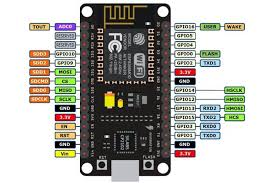
\includegraphics[width=0.5\linewidth]{images/esp 8266.jpg}
    \caption{Modul ESP8266 dengan konfigurasi pin GPIO}
    \label{fig:teori-figure-3}
\end{figure}

\subsection{Konfigurasi Pin dan Fungsionalitas}
Konfigurasi pin ESP8266 dirancang untuk fleksibilitas maksimum dalam berbagai aplikasi IoT. Pin GPIO0 hingga GPIO16 berfungsi sebagai I/O digital dengan kemampuan PWM dan interrupt yang memungkinkan interfacing dengan berbagai sensor dan aktuator. Pin ADC khusus disediakan untuk pembacaan sensor analog yang memerlukan konversi sinyal analog ke digital. Pin TX/RX digunakan untuk komunikasi UART yang memfasilitasi serial debugging dan komunikasi dengan perangkat eksternal. Pin RST berfungsi sebagai reset untuk restart sistem dalam kondisi tertentu, sedangkan pin EN merupakan enable pin untuk aktivasi chip secara keseluruhan. Gambar \ref{fig:teori-figure-3} menunjukkan modul ESP8266 dengan konfigurasi pin GPIO yang lengkap.

\subsection{Pemrograman dan Development Environment}
ESP8266 mendukung berbagai lingkungan pengembangan yang memfasilitasi implementasi aplikasi IoT dengan fleksibilitas tinggi. Arduino IDE dengan ESP8266 Core merupakan platform yang paling populer karena memungkinkan penggunaan sintaks Arduino untuk pemrograman yang familiar bagi sebagian besar developer \citep{monk2016programming}. Framework alternatif yang didukung meliputi ESP-IDF untuk pengembangan tingkat lanjut, MicroPython untuk rapid prototyping, dan NodeMCU Lua untuk pengembangan berbasis scripting. Keberagaman platform ini memungkinkan developer memilih lingkungan yang paling sesuai dengan kebutuhan proyek dan tingkat kompleksitas aplikasi.

\section{\textit{Internet of Things} (IoT)}

\subsection{Definisi dan Konsep Fundamental}
\textit{Internet of Things} (IoT) adalah paradigma komputasi yang memungkinkan objek fisik (\textit{things}) terhubung ke internet dan saling berkomunikasi untuk bertukar data secara otomatis tanpa intervensi manusia \citep{ashton2009internet}. Konsep ini melibatkan integrasi sensor, aktuator, komunikasi nirkabel, dan sistem komputasi awan untuk menciptakan ekosistem digital yang cerdas \citep{ray2018survey}. Implementasi IoT memungkinkan pengumpulan data real-time dari lingkungan fisik, pemrosesan data menggunakan algoritma cerdas, dan respons otomatis terhadap kondisi tertentu.

\subsection{Arsitektur IoT}
Arsitektur IoT umumnya terdiri dari empat lapisan utama yang saling terintegrasi untuk menciptakan sistem yang komprehensif \citep{weber2010governance}. Lapisan persepsi merupakan fondasi sistem yang terdiri dari sensor dan aktuator yang mengumpulkan data lingkungan dan melakukan aksi berdasarkan instruksi yang diterima. Lapisan jaringan menangani transmisi data melalui berbagai protokol komunikasi seperti Wi-Fi, Bluetooth, ZigBee, atau LoRaWAN sesuai dengan kebutuhan aplikasi. Lapisan pemrosesan melakukan analisis dan pemrosesan data menggunakan algoritma yang sesuai, baik secara lokal maupun di cloud computing. Lapisan aplikasi menyediakan interface pengguna dan layanan aplikasi yang memungkinkan interaksi antara pengguna dengan sistem IoT.

\subsection{Protokol Komunikasi IoT}
Sistem IoT menggunakan berbagai protokol komunikasi yang dipilih berdasarkan kebutuhan spesifik aplikasi seperti jangkauan, konsumsi daya, dan throughput data. Wi-Fi IEEE 802.11 digunakan untuk komunikasi lokal berkecepatan tinggi dengan konsumsi daya yang relatif tinggi namun memberikan bandwidth yang luas. Bluetooth dan Bluetooth Low Energy (BLE) cocok untuk komunikasi jarak pendek dengan konsumsi daya rendah, ideal untuk aplikasi wearable dan sensor personal. ZigBee berdasarkan IEEE 802.15.4 dirancang khusus untuk jaringan sensor nirkabel dengan topologi mesh yang dapat mengcover area yang luas. LoRaWAN (Long Range Wide Area Network) dikembangkan untuk komunikasi jarak jauh dengan daya rendah, sangat sesuai untuk aplikasi smart city dan monitoring lingkungan.

\subsection{Message Queuing Telemetry Transport (MQTT)}
MQTT adalah protokol komunikasi \textit{publish-subscribe} yang dirancang khusus untuk aplikasi IoT dengan bandwidth terbatas dan koneksi tidak stabil \citep{zhang2021iot}. Protokol ini beroperasi di atas TCP/IP dan menggunakan arsitektur broker-client yang memungkinkan komunikasi yang efisien dan dapat diandalkan. Desain MQTT memprioritaskan efisiensi bandwidth dan ketahanan terhadap gangguan jaringan, menjadikannya ideal untuk aplikasi IoT yang memerlukan transmisi data real-time dengan konsumsi daya minimal.

\subsubsection{Arsitektur MQTT}
Sistem MQTT terdiri dari tiga komponen utama yang bekerja secara sinergis. Publisher merupakan perangkat yang mengirim data ke broker dengan topik tertentu yang telah ditentukan. Broker berfungsi sebagai server yang menerima, memfilter, dan mendistribusikan pesan kepada subscriber yang berlangganan topik tertentu. Subscriber adalah perangkat yang menerima data dari broker berdasarkan topik yang telah mereka subscribe sebelumnya. Arsitektur ini memungkinkan komunikasi many-to-many yang efisien dan fleksibel.

\subsubsection{Quality of Service (QoS) dalam MQTT}
MQTT mendefinisikan tiga level Quality of Service (QoS) untuk pengiriman pesan yang memberikan fleksibilitas dalam menentukan tingkat keandalan transmisi data \citep{anderson2019digital}. QoS 0 atau \textit{At most once} memungkinkan pesan dikirim maksimal satu kali tanpa konfirmasi, cocok untuk data yang tidak kritis dan dapat mentolerir kehilangan data. QoS 1 atau \textit{At least once} menjamin pesan terkirim minimal satu kali dengan kemungkinan duplikasi, sesuai untuk data penting yang memerlukan konfirmasi penerimaan. QoS 2 atau \textit{Exactly once} menjamin pesan terkirim tepat satu kali tanpa duplikasi, ideal untuk data kritis yang memerlukan integritas tinggi.

\subsubsection{Struktur Topik MQTT}
Topik MQTT menggunakan struktur hierarkis dengan separator "/" untuk mengorganisir data secara sistematis dan logis. Contoh implementasi dalam penelitian ini menggunakan struktur seperti \lstinline|sensor/koefisien_restitusi/bola_tenis/tinggi_awal| dan \lstinline|sensor/koefisien_restitusi/bola_tenis/tinggi_pantul| yang memungkinkan kategorisasi data berdasarkan jenis sensor, parameter yang diukur, objek pengukuran, dan jenis data spesifik.

\begin{verbatim}
sensor/koefisien_restitusi/bola_tenis/tinggi_awal
sensor/koefisien_restitusi/bola_tenis/tinggi_pantul
\end{verbatim}

\section{Karakteristik Material Bola}

\subsection{Klasifikasi Material Berdasarkan Sifat Mekanik}
Material bola dapat diklasifikasikan berdasarkan sifat mekaniknya yang mempengaruhi koefisien restitusi secara signifikan \citep{kalnins2018separation}. Material elastis seperti polimer dengan modulus elastisitas tinggi menunjukkan kemampuan pemulihan bentuk yang baik setelah deformasi, menghasilkan koefisien restitusi yang relatif tinggi. Material viskoelastis termasuk karet alam dan sintetis memiliki karakteristik yang menggabungkan sifat elastis dan viskos, di mana respons terhadap beban bergantung pada waktu dan kecepatan pembebanan. Material komposit yang merupakan kombinasi serat dan matriks polimer menunjukkan sifat mekanik yang dapat disesuaikan berdasarkan orientasi serat dan jenis matriks yang digunakan.

\subsection{Hubungan Modulus Elastisitas dengan Koefisien Restitusi}
Modulus elastisitas ($E$) material didefinisikan sebagai rasio antara tegangan normal ($\sigma$) terhadap regangan normal ($\varepsilon$) yang memberikan ukuran kekakuan material:

\begin{equation}
    E = \frac{\sigma}{\varepsilon}
\end{equation}

dimana:
\begin{itemize}
    \item $E$ = modulus elastisitas (Pa)
    \item $\sigma$ = tegangan normal (Pa)
    \item $\varepsilon$ = regangan normal (tanpa dimensi)
\end{itemize}

Tegangan dan regangan dapat dihitung menggunakan persamaan yang menghubungkan gaya dan deformasi dengan sifat geometris material:

\begin{equation}
    \sigma = \frac{F}{A}
\end{equation}

\begin{equation}
    \varepsilon = \frac{\Delta L}{L_0}
\end{equation}

dimana:
\begin{itemize}
    \item $F$ = gaya yang diterapkan (N)
    \item $A$ = luas penampang ($m^2$)
    \item $\Delta L$ = perubahan panjang (m)
    \item $L_0$ = panjang awal (m)
\end{itemize}

\subsection{Geometri Bola dan Kalkulasi Volume}
Geometri bola memainkan peran penting dalam analisis karakteristik material dan perhitungan parameter fisik. Volume bola ($V$) dihitung menggunakan persamaan geometris fundamental:

\begin{equation}
    V = \frac{4}{3}\pi r^3
\end{equation}

dimana:
\begin{itemize}
    \item $V$ = volume bola (m³)
    \item $r$ = jari-jari bola (m)
    \item $\pi$ = konstanta pi (3.14159...)
\end{itemize}

Luas permukaan bola ($A$) diberikan oleh persamaan yang menentukan area kontak potensial selama tumbukan:

\begin{equation}
    A = 4\pi r^2
\end{equation}

dimana:
\begin{itemize}
    \item $A$ = luas permukaan bola ($m^2$)
\end{itemize}

\subsection{Material Bola dalam Penelitian}
Penelitian ini menggunakan lima jenis bola dengan karakteristik material yang berbeda untuk memberikan variasi yang komprehensif dalam analisis koefisien restitusi \citep{avancini2020physical}. Bola tenis meja terbuat dari selulosa asetat dengan densitas rendah yang memberikan karakteristik pantulan yang responsif dan konsisten. Bola bekel menggunakan karet sintetis dengan elastisitas tinggi yang memungkinkan pemulihan energi yang efisien selama proses tumbukan. Bola plastik terbuat dari polietilena dengan sifat termoplastik yang menunjukkan deformasi plastis yang signifikan selama tumbukan. Bola karet menggunakan karet alam dengan sifat viskoelastis yang memberikan respons yang bergantung pada kecepatan deformasi. Bola baseball menggunakan material komposit berlapis yang menggabungkan berbagai material untuk mengoptimalkan performa dan durabilitas. Setiap material memiliki karakteristik unik yang mempengaruhi respons dinamis selama proses tumbukan, yang tercermin dalam nilai koefisien restitusi yang berbeda untuk setiap jenis bola dan memberikan insight mendalam tentang hubungan antara sifat material dan perilaku tumbukan.